\documentclass{article}
\usepackage[utf8]{inputenc}
\usepackage[T1]{fontenc}
\usepackage[french]{babel}
\usepackage{graphicx}
\usepackage{multicol}
\setlength{\columnsep}{5cm}
\usepackage{hyperref}
\usepackage{textcomp}
\usepackage{gensymb}
\newcommand{\hsp}{\hspace{20pt}}
\newcommand{\HRule}{\rule{\linewidth}{0.5mm}} 
\usepackage{float}
\usepackage{geometry}
\geometry{top=3cm, bottom=3cm, left=3cm, right=3cm}
\usepackage{subcaption}
\usepackage{enumitem}
\usepackage{wrapfig}
\usepackage{algorithm}
\usepackage{algorithmic}
\usepackage{amssymb}
\usepackage{amsmath}
\usepackage{array}
\usepackage{minted}


\begin{document}

%%%%%%%%%%%%%%%%%
% PAGE DE GARDE %
%%%%%%%%%%%%%%%%%

\begin{titlepage}
    \begin{sffamily}
        \begin{center}
            
\includegraphics[scale=0.2]{Logo_Polytech_Sorbonne.png}\\[1.5cm]
            \textsc{\Large \bfseries{Projet Mathématiques Informatique}}\\[1.5cm]
            % Titre
            \HRule \\[0.4cm]
            { \huge \bfseries Sujet 2\\[0.4cm]}
            \HRule \\[2cm]
            
\includegraphics[scale=0.4]{su.png}\\[2cm]
             % Auteurs
            \begin{minipage}{0.4\textwidth}
                \begin{flushleft} \large
                    \textsc{Tristan MICHEL\\ Kenza EL MHAMDI }
                \end{flushleft}
            \end{minipage}
            \begin{minipage}{0.4\textwidth}
                \begin{flushright} \large
                    \textsc{Aissam RABHI\\ Naël SENNOUN}
                \end{flushright}
            \end{minipage}
            \vfill
        
            % Bas de la page
            {\large 2019-2020}
            
        \end{center}
    \end{sffamily}
\end{titlepage}

%%%%%%%%%%%%
% SOMMAIRE %
%%%%%%%%%%%%
\tableofcontents
\newpage

\section*{Introduction}
L'objectif du projet est de modéliser, par le système différentiel \eqref{eq:S} ci-dessous, deux espèces en \\compétitions.

\begin{equation}
\tag{S}
\label{eq:S}
\left\{
\begin{array}{ll}
    \frac{dx}{dt} =  x(1 - \frac{x}{k} - \frac{a y}{k}) \\
    \frac{dy}{dt} = y(1- \frac{y}{l} - \frac{x^{2}}{l})
\end{array}
\right.
\end{equation}\\

Ici $x$ représente le nombre d’individus de la première espèce, $y$ le nombre d’individus de la
deuxième espèce, $k$ est le nombre d’individus de la première espèce que peut nourrir le milieu, $l$ est le nombre d’individus de la deuxième espèce que peut nourrir le milieu et $a$ est un coefficient. Ici, nous reprenons alors l'évolution de ces espèces dans un milieu donné. Le système différentiel \eqref{eq:S} permet de modéliser le problème et de faciliter sa compréhension. Ceci est donc le parfait exemple pour démontrer le rapport entre les mathématiques et l'environnement. En effet, nous nous intéressons à la croissance du nombre d'individus de chaque espèce selon la capacité du milieu à les nourrir.\\

Dans ce projet nous réalisons une étude qualitative de l’évolution du système modélisé. Il s’agit la plupart du temps de déterminer la stabilité de la communauté étudiée, les conditions hypothétiques d’existence d’une stabilité, la sensibilité d’une telle conditions vis à vis des paramètres, des conditions initiales, de la complexité du système.\\

Notre étude sera subdivisée en trois grandes parties :\\

- Pour la première partie, nous allons réaliser une approche théorique qui consiste en une analyse mathématique du problème. \\

- La deuxième partie consistera en l'analyse des graphes obtenus (en Python), ce qui permettra de visualiser l'évolution de chacune des espèces en fonction des différents paramètres.\\

- La troisième et dernière partie sera consacrée à l'interprétation des limites du modèle considéré ainsi qu'aux potentielles améliorations de celui-ci.



\newpage

\setcounter{secnumdepth}{2}
\section{Analyse mathématique}
\subsection{Analyse du modèle}
\vspace{0.4cm}
L’étude que nous allons présenter porte sur la construction et l’analyse de modèles mathématiques pour gérer la croissance ainsi que les interactions entre deux espèces évoluant dans un certain environnement.\\
La variation du nombre d'individus d'une espèce dépend de la capacité du milieu à la nourrir (définie par les coefficients $k$ et $l$). Pour $k$ et $l$ très grands, le terme $(- \frac{x}{k} - \frac{a y}{k})$ sera négligeable, on se retrouve donc avec l'équation : 
\begin{equation*}
\left\{
\begin{array}{ll}
    \frac{dx}{dt} = x \\
    \frac{dy}{dt} = y
\end{array}
\right.
\end{equation*}
\\dont les solutions sont des fonctions exponentielles. \\

On en déduit qu'avec une très grande capacité d'approvisionnement, le nombre d'individu de l'espèce croit de façon exponentielle. \\
Pour un $k$ (ou $l$) quelconque, la variation du nombre d'individu de l'espèce $x$ (ou $y$) dépend du signe de \hspace{0.1cm} $(1 - \frac{x}{k} - \frac{a y}{k})$ \hspace{0.1cm} (respectivement $ (1 -\frac{y}{l} - \frac{x^{2}}{l})$).\\\\\\

\noindent
Pour un instant t fixé, la population augmente a $t + dt$ si :
\begin{equation*}
    k > x(t) + a y(t) \hspace{0.2cm} \text{(ou } l> y(t) + x(t)^{2}) 
\end{equation*}\\
\begin{itemize}
    \item $k$ et $l$ sont les capacités du milieu à nourrir $x$ et $y$
    \item $x$ (respectivement $y$) est le nombre d'individu nourris par le milieu $k$ (resp. $l$)
    \item $a$ est un coefficient (entre 0 et 1) représentant le pourcentage d'individus de $y$ nourris par le milieu $k$
    \item le terme $x + a y$ $(\text{ou } y+ x^{2})$ est la consommation dans $k$ (ou $l$)
    \item lorsque la consommation dépasse la capacité, il n'y a plus assez de provisions et la population de $x$ (ou de $y$) diminue
\end{itemize}

\vspace{1cm}
On peut interpréter cette inégalité de la manière suivante :\\

Si l'on se place dans le cas idéal c'est à dire qu'on se place dans le cas où le milieu dispose d'assez de ressources pour couvrir les besoins vitaux des deux espèces considérés. La population va donc croître de façon exponentielle, ce qui outre l'hypothèse des ressources infinies contredit les observations. Or si la densité d'une des deux espèces est trop forte, les individus vont se retrouver en compétition. On parle alors de croissance densité dépendante ou logistique.\\

\vspace{0.5cm}
Celle-ci peut être représentée par :
\begin{equation}
\label{eq:g}
\tag{G}
    g(P) = (\lambda-kP(t))
\end{equation}
où $k$ est appelé coefficient logistique de la population et $g(P)$ est une fonction polynomiale en $P$ appelée taux de croissance.
On pose : 
\begin{equation*}
    K = \frac{\lambda}{k}= \frac{f-m}{k}
\end{equation*}\\

Avec $f$ : taux de fertilité et $m$ : taux de mortalité.\\

La solution de l'équation \eqref{eq:g} s'écrit :

\begin{equation*}
    P(t) = \frac{P_{0}K}{P_{0}+(K-P_{0})\exp{-\lambda}t}
\end{equation*}\\

Et par suite, on a :\\

\noindent
- Si $\lambda > 0$, alors on a $P(t) \longrightarrow 0$ quand $t \longrightarrow \infty$\\

\noindent
- Si $\lambda \leqslant 0$, alors on a $P(t) \longrightarrow K$ quand $t \longrightarrow \infty$\\


\noindent
- Or on a $P(t) = K$ une solution stationnaire car $P(t)$ est décroissante si $K < P_0$ et croissante sinon\\

En effet, lorsque en absence de compétition entre les deux espèces, la densité de la population atteint la valeur K que l'on appelle capacité d'accueil du milieu.\\

Étudier le comportement de l'écosystème en fonction des différents paramètres, essayer de trouver un équilibre entre deux espèces en compétition dans un même milieu est ce qu'on cherche à déterminer.\\

On va alors d'abord commencer par l'étude qualitative du système suivant :\\
\vspace{1cm}
\begin{equation}
\tag{S}
\left\{
\begin{array}{cc}
   x' =  x(1 - \frac{x}{k} - \frac{a y}{k}) \\\\
   y' = y(1- \frac{y}{l} - \frac{x^{2}}{l})
\end{array}
\right.
\end{equation}

\newpage

\subsection{Analyse de la stabilité}
On s'intéresse d'abord au potentiels points d'équilibre du système, les deux populations seront à l'équilibre lorsqu'elles arrêteront de varier i.e x' = 0 et y' = 0. Ce qui veut dire qu'en partant avec des conditions initiales qui vérifie $(x_{0},y_{0}) = (P1, P2)$
avec P1 = coordonnée en x du point fixe et P2 = coordonnée en y du point fixe, il n'y a aucune variation des populations.
\subsubsection{Définition des points fixes}

Le problème donné est un système non linéaire, on cherche les points singuliers du système en résolvant l'équation $f(x,y) = (0,0) $ avec :
\begin{equation*}
    f(x,y) = 
    \begin{pmatrix}
        \quad x(1 - \frac{x}{k} - \frac{a y}{k})\phantom{\quad}\\\\
        \quad y(1- \frac{y}{l} - \frac{x^{2}}{l})\phantom{\quad}
    \end{pmatrix}
\end{equation*}

\vspace{0.5cm}
On a un système d'équations du second ordre à résoudre :\\
\begin{equation}
\label{eq:f1}
\tag{S.F}
\left\{
    \begin{array}{ll}
        x(1 - \frac{x}{k} - \frac{a y}{k}) & = 0 \\
        y(1- \frac{y}{l} - \frac{x^{2}}{l}) & = 0
    \end{array}
\right.
\hspace{0.5cm}
\Leftrightarrow
\hspace{0.5cm}
\left\{
    \begin{array}{ll}
        x = 0 \quad \text{ou} & x = k - a y \\
        y = 0 \quad \text{ou} & y = l - x^2
    \end{array}
\right.
\end{equation}\\

\vspace{0.5cm}
On peut donc déterminer plusieurs points fixe:\\\\
\phantom{}\hfill $(0,0)$ \hfill $(0,l - x^2) = (0,l)$ \hfill $(- a y + k,0) = (k,0)$ \hfill $(k - a y, l - x^{2})$ \hfill \phantom{}\\

\vspace{0,5cm}
On calcule maintenant les coordonnées de ce dernier points en fonction des paramètres.\\
\begin{equation}
\label{eq:f2}
\tag{S.F2}
\left\{
    \begin{array}{l}
        x = k - ay \\
        y = l - x^{2}
    \end{array}
\right.
\hspace{0.5cm}
\Leftrightarrow
\hspace{0.5cm}
\left\{
    \begin{array}{l}
        ax^{2} - x - al + k = 0\\
        y = l - x^{2}
    \end{array}
\right.
\end{equation}\\
\vspace{0,5cm}

Le système \eqref{eq:f2} admet des solutions dans $\mathbb{R}$, on peut donc en déduire :
\begin{equation*}
\begin{array}{cc}
    x\ =\ \dfrac{1 \pm \sqrt{\Delta}}{2a} \qquad \text{avec} \qquad \Delta\ =\ 1 + 4a(al -k)\ \geqslant\ 0\\\\
    \implies
    x\ =\ \dfrac{1 \pm \sqrt{1 + 4a(al - k)}}{2a}
    \qquad \text{et} \qquad
    y\ =\ \dfrac{k}{a} - \dfrac{1 \pm \sqrt{1 + 4a(al -k)}}{2a^2}
\end{array}
\end{equation*}\\

\newpage
- Si $\Delta > 0\ \Leftrightarrow\ a > \frac{k + \sqrt{k^2 - l} }{2l}$, alors le système \eqref{eq:f2} admet deux solution qui sont : 
\begin{equation*}
    \left(\ \dfrac{1 + \sqrt{1 + 4a(al -k)}}{2a}\ ,\ \dfrac{k}{a} - \dfrac{1 + \sqrt{1 + 4a(al -k)}}{2a^2}\ \right)
    \text{ et }
    \left(\ \dfrac{1 - \sqrt{1 + 4a(al -k)}}{2a}\ ,\ \dfrac{k}{a} - \dfrac{1 - \sqrt{1 + 4a(al -k)}}{2a^2}\ \right)
\end{equation*}\\

\qquad Donc les points critiques sont :
$\qquad (0,0),\quad (0,l),\quad (k,0),$\\

$\phantom{} \hfill \left(\frac{1 + \sqrt{1 + 4a(al -k)}}{2a}, \frac{k}{a} - \frac{1 + \sqrt{1 + 4a(al -k)}}{2a^2} \right),
\quad \left(\frac{1 - \sqrt{1 + 4a(al -k)}}{2a}, \frac{k}{a} - \frac{1 - \sqrt{1 + 4a(al -k)}}{2a^2}\right) \hfill$\\

\vspace{1cm}
- Si $\Delta < 0\ \Leftrightarrow\ a < \frac{k}{2l}$, alors le système \eqref{eq:f2} n'admet pas de solution réelle.\\

Donc les points critiques sont : $\qquad (0,0),\quad (0,l),\quad (k,0)$ \\

\vspace{1cm}
- Si $\Delta = 0\ \Leftrightarrow\ a = \frac{k + \sqrt{k^2 - l} }{2l}\ \text{et}\ k \geqslant \sqrt{l}$, alors le système \eqref{eq:f2} admet une solution : 
\begin{equation*}
    \left(\ \dfrac{l}{k + \sqrt{k^2 - l}},\ l\left(1 - \dfrac{l}{(k + \sqrt{k^2 - l})^2} \right)\ \right)
\end{equation*}
\qquad Donc les points critiques sont : $\qquad (0,0),\quad (0,l),\quad (k,0), \\\\
\phantom{} \hfill \left(\ \frac{l}{k + \sqrt{k^2 - l}},\ l\left(1 - \frac{l}{(k + \sqrt{k^2 - l})^2} \right)\ \right) \hfill$

\newpage
\subsubsection{Stabilité des points d'équilibre}
\noindent
Pour identifier la stabilité de nos points fixes,  on pose $A$ la matrice jacobienne du système.\\

\begin{equation*}
    J_{F}(x,y) = A =
    \begin{pmatrix}
        \ 1- \frac{ay}{k} - \frac{2x}{k} & - \frac{ax}{k}\ \\\\
        \ - \frac{2xy}{l}  & 1 - \frac{x^{2}}{l} - \frac{2y}{l}\ 
    \end{pmatrix}
\end{equation*}\\

\noindent
La détermination de la stabilité consiste en l'observation du signe de la partie réelle des valeurs propres de A en ses points singuliers.\\

\vfill
\noindent
- Pour (0,0):
\begin{equation*}
    A =
    \begin{pmatrix}
        \ 1 & 0 \phantom{\ }\\
        \ 0 & 1 \phantom{\ }
    \end{pmatrix}
\end{equation*}\\
Cette matrice possède une valeur propre double : 1 , le point correspondant est instable.\\

\vfill
\noindent
- Pour (0,$l$) :
\begin{equation*}
    A = 
    \begin{pmatrix}
        \ 1- \frac{al}{k}  & 0 \phantom{\ }\\\\
        \ 0  & -1 \phantom{\ }
    \end{pmatrix}
\end{equation*}\\
Les valeurs propres sont racines de $(-1 - \lambda)(1- \frac{al}{k} - \lambda)$ : soit $\lambda = -1 \text{ et } \lambda = 1 - \frac{al}{k}$\\\\
Grâce à ces valeurs propres nous pouvons caractériser la stabilité de notre point fixe, pour cela il nous a fallu dans un des cas déterminer une fonction de Liapounov $L(x,y) = |y - l|$ qui nous a permit de démontrer la stabilité asymptotique de ce point fixe.
\begin{itemize}
    \item le point est asymptotiquement stable si $al \geqslant k$
    \item le point est instable si $al < k$
\end{itemize}


\vfill
\noindent
- Pour ($k$,0) :
\begin{equation*}
    A =
    \begin{pmatrix}
        \ -1 & -a \phantom{\ }\\\\
        \ 0 & 1 - \frac{k^{2}}{l} \phantom{\ }
    \end{pmatrix}
\end{equation*}\\
Les valeurs propres sont racines de $(\lambda + 1)(\lambda - 1 + \frac{k^2}{l})$ : soit $\lambda = -1 \text{ et } \lambda = 1 - \frac{k^2}{l}$\\\\
Grâce à ces valeurs propres nous pouvons déterminer la stabilité de notre point fixe, pour cela il nous a fallu dans un des cas déterminer une fonction de Liapounov $L(x,y) = |x - k|$ qui nous a permit de démontrer la stabilité asymptotique de ce point fixe.
\begin{itemize}
    \item le point est asymptotiquement stable si $k \geqslant \sqrt{l}$
    \item le point est non stable si $k < \sqrt{l}$
\end{itemize}

\newpage

\vfill
\noindent
- Pour $\left(\frac{1 + \sqrt{1 + 4a(al -k)}}{2a}, \frac{k}{a} - \frac{1 + \sqrt{1 + 4a(al -k)}}{2a^2} \right)$ :
\begin{equation*}
    A = -
    \begin{pmatrix}
        \ \frac{1 + \sqrt{1 + 4a(al -k)}}{2ak} & \frac{1 + \sqrt{1 + 4a(al -k)}}{2k} \phantom{\ }\\\\
         \ \frac{1 + \sqrt{1 + 4a(al -k)}}{a^2 l}(k - \frac{1}{a}) - \frac{2}{a} + \frac{2k}{a^2 l} & \frac{k}{al} - \frac{1 + \sqrt{1 + 4a(al -k)}}{2a^2 l} \phantom{\ }
    \end{pmatrix}
\end{equation*}

Les valeurs propres de cette matrice sont racines du polynôme $P(\lambda)$ :
\begin{equation*}
\begin{array}{l}
    \left(\lambda + \frac{1 + \sqrt{1 + 4a(al -k)}}{2ak}\right)
    \left( \lambda + \frac{k}{al} - \frac{1 + \sqrt{1 + 4a(al -k)}}{2a^2 l} \right)
    - \frac{1+\sqrt{1 + 4a(al -k)}}{2k} \cdot \left( \frac{1 + \sqrt{1 + 4a(al -k)}}{a^2 l} \cdot \left(k - \frac{1}{a} \right) - \frac{2}{a} + \frac{2k}{a^2 l} \right)
\end{array}
\end{equation*}

Soit $ P(\lambda)= \alpha \lambda^{2} - \beta \lambda + \gamma$ avec : 

\begin{equation*}
\left \{
\begin{array}{l}
     \alpha = 1\\\\
     \beta =  \frac{k}{al} + \frac{1 + \sqrt{1 + 4a(al -k)}}{2a} \cdot \left( \frac{1}{k} - \frac{1}{al} \right) \\\\
     \gamma = \frac{1 + \sqrt{1 + 4a(al -k)}}{2a^2 l} \cdot \left( \frac{1}{ak} - 3 \right) + \frac{ak - 1}{a^2 l} + \frac{2 + \sqrt{1 + 4a(al -k)}}{ak} - 1\\
\end{array}
\right.
\end{equation*}\\

Ainsi on peut construire la valeur $ \Delta = \beta^2 - 4 \alpha \gamma $, soit :\\ 
\begin{equation}
    \tag{ \Delta }
    \label{pt5:delta}
    \begin{array}{ll}
        \Delta = \frac{1 + \sqrt{1 + 4a(al -k)}}{a} \cdot \left( \frac{1}{al} \cdot \left( 4 - \frac{2k-1}{2al} - \frac{a+1}{ak} \right) + \frac{1-8k}{2k^2} \right) + \frac{a^2 l - k (3a+4)}{ak^2} + \frac{k(k-1) + al(1-4k) + 4l}{a^2 l^2} + 4 \\
    \end{array}
\end{equation}



\vfill
\noindent
- Dans la cas ou $\Delta > 0$\\

Les valeurs propres de la matrice A pour ce point sont  : 
\begin{equation*}
    \left \{
    \begin{array}{l}
        \lambda_{1} = \frac{- \beta - \sqrt{\beta^{2} - 4 \alpha \gamma}}{2\alpha}\\\\
        \lambda_{2} = \frac{- \beta + \sqrt{\beta^{2} - 4 \alpha \gamma}}{2\alpha} 
    \end{array}
    \right.
\end{equation*}
\begin{equation*}
    \Leftrightarrow
    \tiny
    \left \{
    \begin{array}{l}
        \lambda_{1} =  - \frac{k}{2al} + \frac{1 + \sqrt{1 + 4a(al -k)}}{4a} \cdot \left( \frac{1}{al} - \frac{1}{k} \right) - 
        \frac{1}{2} \sqrt{\frac{1 + \sqrt{1 + 4a(al -k)}}{a} \cdot \left( \frac{1}{al} \cdot \left( 4 - \frac{2k-1}{2al} - \frac{a+1}{ak} \right) + \frac{1-8k}{2k^2} \right) + \frac{a^2 l - k (3a+4)}{ak^2} + \frac{k(k-1) + al(1-4k) + 4l}{a^2 l^2} + 4}
        \\\\
        \lambda_{2} = - \frac{k}{2al} + \frac{1 + \sqrt{1 + 4a(al -k)}}{4a} \cdot \left( \frac{1}{al} - \frac{1}{k} \right) +
        \frac{1}{2} \sqrt{\frac{1 + \sqrt{1 + 4a(al -k)}}{a} \cdot \left( \frac{1}{al} \cdot \left( 4 - \frac{2k-1}{2al} - \frac{a+1}{ak} \right) + \frac{1-8k}{2k^2} \right) + \frac{a^2 l - k (3a+4)}{ak^2} + \frac{k(k-1) + al(1-4k) + 4l}{a^2 l^2} + 4}
        \\
    \end{array}
    \right.
\end{equation*}

La stabilité du point fixe dépend du signe des parties réelles des valeurs propres.\\
\begin{equation*}
\left \{
    \begin{array}{llll}
        Re(\lambda_{1}) < 0 &
        \quad \Leftrightarrow \quad \lambda_{1} < 0 &
        \quad \Leftrightarrow \quad \beta + \sqrt{\beta^{2} - 4 \alpha \gamma} > 0 &
        \quad \Leftrightarrow \quad \beta > 0 \\\\
        Re(\lambda_{2}) < 0 &
        \quad \Leftrightarrow \quad \lambda_{2} < 0 &
        \quad \Leftrightarrow \quad \beta > \sqrt{\beta^{2} - 4 \alpha \gamma} &
        \quad \Leftrightarrow \quad \gamma > 0 \\
    \end{array}
\right.
\end{equation*}

Tant que $\gamma > 0$, le point est asymptotiquement stable.
Sinon il est instable.

\vfill
\noindent
- Dans la cas ou $\Delta \leqslant 0$\\

La partie réelle des valeurs propres de la matrice A pour ce point est : 
\begin{equation*}
    \begin{array}{lll}
        Re(\lambda_{0,1,2}) = - \frac{\beta}{2\alpha} < 0 &
        \Leftrightarrow &
        \beta > 0
    \end{array}
\end{equation*}

Ce point est donc asymptotiquement stable si $\beta > 0$. Sinon il est non stable.


\newpage

\vfill
\noindent
- Pour $\left(\frac{1 - \sqrt{1 + 4a(al -k)}}{2a}, \frac{k}{a} - \frac{1 - \sqrt{1 + 4a(al -k)}}{2a^2}\right)$ :
\begin{equation*}
    A = -
    \begin{pmatrix}
        \ \frac{1 - \sqrt{1 + 4a(al -k)}}{2ak} & \frac{1 - \sqrt{1 + 4a(al -k)}}{2k} \phantom{\ }\\\\
        \ \frac{1 - \sqrt{1 + 4a(al -k)}}{a^2 l}(k - \frac{1}{a}) - \frac{2}{a} + \frac{2k}{a^2 l} & \frac{k}{al} - \frac{1 - \sqrt{1 + 4a(al -k)}}{2a^2 l} \phantom{\ }
    \end{pmatrix}
\end{equation*}

\begin{equation*}
    det_{\lambda I_2 - A} = 
    \left|
    \begin{array}{lr}
       \ \lambda + \frac{1 - \sqrt{1 + 4a(al -k)}}{2ak} & \frac{1 - \sqrt{1 + 4a(al -k)}}{2k} \phantom{\ }\\\\
        \ \frac{1 - \sqrt{1 + 4a(al -k)}}{a^2 l}(k - \frac{1}{a}) - \frac{2}{a} + \frac{k}{a^2 l} & \lambda + \frac{k}{al} - \frac{1 - \sqrt{1 + 4a(al -k)}}{2a^2 l} \phantom{\ }
    \end{array}
    \right|
\end{equation*}

Les valeurs propres de cette matrice sont racines du polynôme $P(\lambda)$ :
\begin{equation*}
\begin{array}{l}
    \left(\lambda + \frac{1 - \sqrt{1 + 4a(al -k)}}{2ak}\right)
    \left( \lambda + \frac{k}{al} - \frac{1 - \sqrt{1 + 4a(al -k)}}{2a^2 l} \right)
    - \frac{1-\sqrt{1 + 4a(al -k)}}{2k} \cdot \left( \frac{1 - \sqrt{1 + 4a(al -k)}}{a^2 l} \cdot \left(k - \frac{1}{a} \right) - \frac{2}{a} + \frac{2k}{a^2 l} \right)
\end{array}
\end{equation*}

Soit $ P(\lambda)= \alpha \lambda^{2} - \beta \lambda + \gamma$ avec : 
\begin{equation*}
\left \{
\begin{array}{l}
     \alpha = 1\\\\
     \beta =  \frac{k}{al} + \frac{1 - \sqrt{1 + 4a(al -k)}}{2a} \cdot \left( \frac{1}{k} - \frac{1}{al} \right) \\\\
     \gamma = \frac{1 - \sqrt{1 + 4a(al -k)}}{2a^2 l} \cdot \left( \frac{1}{ak} - 3 \right) + \frac{ak - 1}{a^2 l} + \frac{2- \sqrt{1 + 4a(al -k)}}{ak} -1 \\
\end{array}
\right.
\end{equation*}\\

Ainsi on peut construire la valeur $ \Delta = \beta^2 - 4 \alpha \gamma $, soit :
\begin{equation*}
\tag{ \Delta }
\label{pt4:delta}
    \begin{array}{l}
        \Delta = \frac{1 - \sqrt{1 + 4a(al -k)}}{a} \cdot \left( \frac{1}{al} \cdot \left( 4 - \frac{2k-1}{2al} - \frac{a+1}{ak} \right) + \frac{1-8k}{2k^2} \right) + \frac{a^2 l - k (3a+4)}{ak^2} + \frac{k(k-1) + al(1-4k) + 4l}{a^2 l^2} + 4 \\
    \end{array}
\end{equation*}


\noindent
- Dans le cas où $\Delta > 0$\\\\ Les valeurs propres sont : 
\begin{equation*}
\left \{
    \begin{array}{l}
        \lambda_{1} = \frac{- \beta - \sqrt{\beta^{2} - 4 \alpha \gamma}}{2\alpha}\\\\
        \lambda_{2} = \frac{- \beta + \sqrt{\beta^{2} - 4 \alpha \gamma}}{2\alpha}
    \end{array}
\right.
\end{equation*}

\begin{equation*}
\Rightarrow 
\tiny
\left \{
    \begin{array}{l}
        \lambda_{1} =   \frac{-k}{2al} - \frac{1 - \sqrt{1 + 4a(al -k)}}{4a} \cdot \left( \frac{1}{k} - \frac{1}{al} \right) -  \frac{1}{2} \sqrt{ \left(  \frac{k}{al} + \frac{1 - \sqrt{1 + 4a(al -k)}}{2a} \cdot \left( \frac{1}{k} - \frac{1}{al} \right) \right)  ^{2} - \left(    \frac{4 - 4\sqrt{1 + 4a(al -k)}}{2a^2 l} \cdot \left( \frac{1}{ak} - 3 \right) + \frac{4(ak - 1)}{a^2 l} + \frac{8 - 4\sqrt{1 + 4a(al -k)}}{ak} - 4    \right)    }\\\\
        
        \lambda_{2} =  \frac{-k}{2al} - \frac{1 - \sqrt{1 + 4a(al -k)}}{4a} \cdot \left( \frac{1}{k} - \frac{1}{al} \right) + \frac{1}{2} \sqrt{ \left(  \frac{k}{al} + \frac{1 - \sqrt{1 + 4a(al -k)}}{2a} \cdot \left( \frac{1}{k} - \frac{1}{al} \right) \right)  ^{2} + \left(    \frac{4 - 4\sqrt{1 + 4a(al -k)}}{2a^2 l} \cdot \left( \frac{1}{ak} - 3 \right) + \frac{4(ak - 1)}{a^2 l} + \frac{8 - 4\sqrt{1 + 4a(al -k)}}{ak} - 4    \right)    } \\
    \end{array}
\right.
\end{equation*} 
La stabilité du point critique étudié dépend du signe de la partie réelle des valeurs propres. $\lambda_1$ étant négatif, on cherche à déterminer le signe de $\lambda_2$.

\begin{equation*}
    \begin{array}{cc}
        \frac{- \beta + \sqrt{\beta^{2} - 4 \alpha \gamma}}{2\alpha} < 0 
        \iff \sqrt{\beta^{2} - 4 \gamma } < \beta \\\\ \iff
        \beta^{2} - 4 \gamma < \beta^{2}  \iff
        -4 \gamma < 0 \\\\ \iff
        \gamma > 0 
    \end{array}
\end{equation*}
Le point est  asymptotiquement stable  si on choisit des paramètres $a,k$ et $l$ tel que $\gamma$ soit positif, on vérifiera la valeur de ce dernier avant la mise en oeuvre.
\newpage
\noindent
- Pour $\left(\ \frac{l}{k + \sqrt{k^2 - l}},\ l\left(1 - \frac{l}{(k + \sqrt{k^2 - l})^2} \right)\ \right)$ :
\begin{equation*}
    A = -
    \begin{pmatrix}
        \ \frac{l}{k^2 + k\sqrt{k^2 - l}} & \frac{al}{k^2 + k\sqrt{k^2 - l}} \phantom{\ }\\\\
        \ \frac{2l}{k + \sqrt{k^2 - l}} \cdot (1 - \frac{l}{(k + \sqrt{k^2 - l})^2}) & 1 - \frac{l}{(k + \sqrt{k^2 - l})^2} \phantom{\ }
    \end{pmatrix}
\end{equation*}
Calcul des racines du polynôme caractéristique, et en remplaçant $a$ par sa valeur : 
\begin{equation*}
    P(\lambda) = det_{A} = 
    \left|
    \begin{array}{lr}
        -\frac{l}{k^2 + k\sqrt{k^2 - l}} - \lambda & -\frac{1}{2k}  \\ \\
        -\frac{2l}{k + \sqrt{k^2 - l}} \cdot (1 - \frac{l}{(k + \sqrt{k^2 - l})^2}) & \frac{l}{k + \sqrt{k^2 - l}}- 1 -\lambda 
    \end{array}
    \right|
\end{equation*} \\
On cherche donc les racines de $P(\lambda)$
\begin{equation}
\tag{P}
    P(\lambda)  = (\dfrac{l}{k^2+k\sqrt{k^2-l}}+\lambda)(1+\lambda-\frac{l}{k+\sqrt{k^2-l}})-\dfrac{l}{k^2+k\sqrt{k^2-l}}(1-\frac{l}{(k+\sqrt{k^2-l)^2}})
\end{equation}

\begin{equation*}
    = \alpha \lambda^{2} + \beta \lambda + \gamma \text{\quad avec : \qquad}
    \left \{
    \begin{array}{l}
        \alpha =  1\\\\ 
        \beta =   \frac{k^{2} + l(1-k) + k \sqrt{k^{2} - l}}{k(k + \sqrt{k^{2} })}\\\\
        \gamma =  \frac{l (lk(k+\sqrt{k^{2}-l}))}{k^{2}( k + \sqrt{k^{2} - l})^{3} }\\ 
    \end{array}
\right.
\end{equation*}


\begin{equation}
    \tag{ \Delta }
    \begin{array}{l}
       \Delta = \frac{1 + \sqrt{1 + 4a(al -k)}}{a} \cdot \left( \frac{1}{al} \cdot \left( 4 - \frac{2k-1}{2al} - \frac{a+1}{ak} \right) + \frac{1-8k}{2k^2} \right) + \frac{a^2 l - k (3a+4)}{ak^2} + \frac{k(k-1) + al(1-4k) + 4l}{a^2 l^2} + 4 \\
    \end{array}
    \label{pt6:delta}
\end{equation}


On détermine alors la valeurs propres de la matrice en fonction du signe de $\Delta = \beta^{2} - 4\alpha \gamma$ \\ les valeurs propres de la matrice A pour ce point sont : \\\\
\noindent
- Dans le cas $\Delta > 0$

\begin{equation*}
    \left \{
    \begin{array}{l}
        \lambda_{1} = \frac{- \beta - \sqrt{\beta^{2} - 4 \alpha \gamma}}{2\alpha}\\\\
        \lambda_{2} = \frac{- \beta + \sqrt{\beta^{2} - 4 \alpha \gamma}}{2\alpha} 
    \end{array}
    \right.
    \Rightarrow\ 
    \left \{
    \begin{array}{l}
        \lambda_{1} = -\frac{1}{2} \left(   \frac{k^{2} + l(1-k) + k \sqrt{k^{2} - l}}{k(k + \sqrt{k^{2} })}  + \sqrt{ ( \frac{k^{2} + l(1-k) + k \sqrt{k^{2} - l}}{k(k + \sqrt{k^{2} })} )^{2} -   \frac{4l (lk(k+\sqrt{k^{2}-l})}{k^{2}( k + \sqrt{k^{2} - l})^{3} }    } \right) \\\\
        \lambda_{2} = -\frac{1}{2} \left(   \frac{k^{2} + l(1-k) + k \sqrt{k^{2} - l}}{k(k + \sqrt{k^{2} })}  - \sqrt{ ( \frac{k^{2} + l(1-k) + k \sqrt{k^{2} - l}}{k(k + \sqrt{k^{2} })} )^{2} -   \frac{4l (lk(k+\sqrt{k^{2}-l})}{k^{2}( k + \sqrt{k^{2} - l})^{3} }    } \right)
    \end{array}
    \right.
\end{equation*}
La stabilité de ce point singulier dépend du signe de $\lambda_{1}$ et $\lambda_{2}$. On voit que $\lambda_{1} <0$, on détermine le signe de $\lambda_{2}$

\begin{equation*}
    \begin{array}{ll}
        \frac{- \beta + \sqrt{\beta^{2} - 4 \alpha \gamma}}{2\alpha} < 0 \\ \\
        \iff \sqrt{\beta^{2} - 4 \gamma } < \beta \\ \\ \iff
        \beta^{2} - 4 \gamma < \beta^{2} \\\\ \iff
        -4 \gamma < 0 \\\\ \iff
        \gamma > 0 
    \end{array}
\end{equation*}
Or, $\gamma$ est strictement positif, on en déduis que la valeur propre $\lambda_{2}$ est strictement négative. Donc le point critique est asymptotiquement stable.
\newpage
\noindent
- Dans le cas $\Delta \leqslant 0$ : \\ \\ 
On ne regarde que la partie réelle des valeurs propres de $A$.

\begin{equation*}
    Re (\lambda_{1}) = Re(\lambda_{2}) = - \frac{\beta}{2\alpha} 
\end{equation*}
On a là une valeur propre double dont le signe dépend uniquement de $\beta =  \frac{k^{2} + l(1-k) + k \sqrt{k^{2} - l}}{k(k + \sqrt{k^{2} })}$ \\ \\
On voit que $\beta > 0$ donc les parties réelles des valeurs propres sont strictement négatives. Le point critique est asymptotiquement stable, et ce quelque soit le signe de $\Delta $ (donc $ \forall  (k,l)\in \mathbb{R}^{+}_{*})$\\\\

\subsubsection{Bilan des points critiques:}
\noindent
-$(0,0)$ : Point instable, quelque soient les valeurs des paramètres.\\\\

\noindent
-$(0,l)$ : Point asymptotiquement stable pour $ a \geqslant \frac{k}{l} $, instable sinon.\\\\

\noindent
-$(k,0)$ : Point asymptotiquement stable pour $ k \geqslant \sqrt{l} $, instable sinon.\\\\

\noindent
-$\left(\frac{1 + \sqrt{1 + 4a(al -k)}}{2a}, \frac{k}{a} - \frac{1 + \sqrt{1 + 4a(al -k)}}{2a^2} \right)$ : 
\begin{tabular}{l}
    Point asymptotiquement stable pour $\beta > 0$ avec \\
    en plus $\gamma > 0$ si $\Delta > 0$, instable sinon.
\end{tabular}\\\\\\

\noindent
-$\left(\frac{1  - \sqrt{1 - 4a(al -k)}}{2a}, \frac{k}{a} - \frac{1 - \sqrt{1 + 4a(al -k)}}{2a^2} \right)$ :
\begin{tabular}{l}
    Point asymptotiquement stable pour $\beta > 0$ avec \\ en plus $\gamma > 0$ si $\Delta >0$ instable sinon.
\end{tabular}\\\\

\noindent
-$\left(\ \frac{l}{k \\+ \sqrt{k^2 - l}},\ l\left(1 - \frac{l}{(k + \sqrt{k^2 - l})^2} \right)\ \right)$ : 
\begin{tabular}{l}
Point asymptotiquement stable pour tout $(k,l) \in \mathbb{R}_+^*$\\
avec $a = \frac{k + \sqrt{k^2 - l} }{2l}\ \text{et}\ k \geqslant \sqrt{l}$\\
\end{tabular}\\\\\\

\newpage
\setcounter{secnumdepth}{2}
\newpage
\section{Mise en oeuvre}
\vspace{0.5cm}
\subsection{Explication de l'outil Python}
\vspace{0.5cm}
Nous avons construit cette application en Python pour le TP $n^o$3 de notre cours de Programmation Python \& Fortran. Elle consiste en un outils capable de représenter graphiquement un système d'équations différentielles. Pour cela il suffit de construire une classe qui représentera notre modèle. Cette classe devra hériter de la classe \verb|AutomoneSys| située dans le fichier \verb|AutonomSys.py|. \\
Ici en exemple le modèle demandé :
\vspace{0.5cm}

\begin{minted}[frame=lines,framesep=2mm,baselinestretch=1.2,linenos]{python}
from mdl.AutonomSys import AutonomSys

class ModelSelectionNaturelle(AutonomSys):
    """ La classe ModelSelectionNaturelle : 
    pour la gestion d'un modèle de proies-prédateurs. """

    @staticmethod
    def system(z, t, args):
        x, y = z[:2]
        dxdt = x * (1 - (x + args["alpha"] * y) / args["k"])
        dydt = y * (1 - (y + x**2) / args["l"])
        return [ dxdt , dydt ]
\end{minted}

\vspace{0.5cm}
Pour intégrer un nouveau système d'équations il suffit juste d'écrire le jeu d'équations dans la classe et on peut directement étudier le modèle.
Si on souhaite faire varier les paramètres d'application de celui-ci, il suffit de changer les caractéristiques que l'on lui applique dans la fonction \verb|main| situé dans le fichier \verb|main.py|.
\vspace{0.5cm}

\begin{minted}[frame=lines,framesep=2mm,baselinestretch=1.2,linenos]{python}
from tools.axis.Axis import Axis
from tools.cnds_initials.Initials import Initials
from tools.line_style_form.Color import Color
from tools.line_style_form.Form import Form
from tools.line_style_form.LineStyle import LineStyle
from tools.phase_diag.PhaseDiag import PhaseDiag
from mdl.ModelSelectionNaturelle import ModelSelectionNaturelle

def main():

    # -- Le modèle
    args = {"alpha": 0.5, "k": 100, "l": 100}
    mdl = ModelSelectionNaturelle(title = "Model Selection Naturelle", args = args)

    # -- Les axes
    xaxis = Axis(label = "x", inf = 0, sup = 100, nbpts = 50)
    yaxis = Axis(label = "y", inf = 0, sup = 100, nbpts = 50)
    taxis = Axis(inf = 0, sup = 100000, nbpts = 10000000)

    # -- Couleurs et formes
    col = Color()
    frm = Form()
    red_solid = LineStyle(color = col.red())
    blue_dashdot = LineStyle(color = col.blue(), form = frm.dash_dot())
    black_dash = LineStyle(color = col.black(), form = frm.dashed())
    
    # -- Conditions initiales
    cnds = Initials(Lx = [10], Ly = [120], style = black_dash)
    cnds.append(coord = (20, 200), style = blue_dashdot)
    cnds.append(coord = (150, 200), style = red_solid)

    # -- Portrait des phases
    phases = PhaseDiag(title = mdl.title)
    phases.portrait(modl = mdl, xaxis = xaxis, yaxis = yaxis, taxis = taxis, listcnd = cnds, exportpng = True) 

if __name__ == '__main__':
    main()
\end{minted}

\vspace{0.5cm}
Ainsi on peut faire varier les différents paramètres qui constituent notre modèle afin d'avoir un modèle perfectionné qui correspond à notre recherche.\\
Après avoir exécuté ce script, le programme affiche son résultat grâce à la librairie \verb|mathplotlib.pyplot| et sauvegarde cet affichage dans le dossier \verb|img/|.

\newpage
\subsection{Illustration des résultats}
Nous allons maintenant illustrer les hypothèses que nous avons établies lors de l'analyse du modèle. En effet, en fonction de celles-ci plusieurs situations  peuvent être représentées.

\subsubsection{Premier cas}
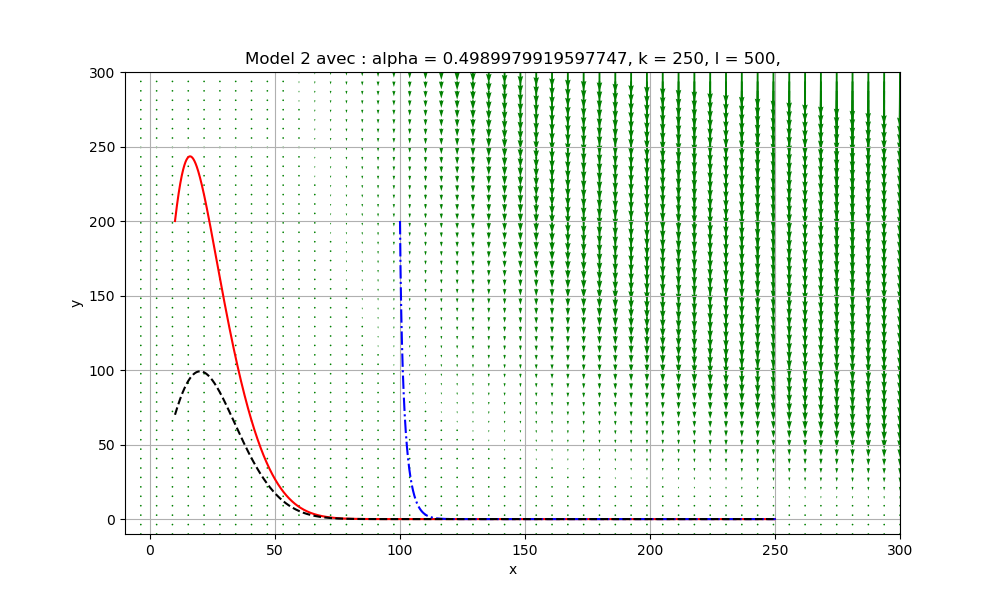
\includegraphics[width = 13cm]{x_predom2.png}\\
On a choisi trois différentes conditions initiales pour montrer que le comportement asymptotique du modèle ne dépend pas de ces dernières. On remarque que pour une valeur de $k\geqslant \sqrt(l)$, c'est bien l'espèce x qui prend le dessus, le système converge alors vers le point stable correspondant. À noter que le nombre d'individus de l'espèce x se limite à 250, cela correspond à la valeur de k. $(x(t),y(t)) \longrightarrow (k,0) $

\subsubsection{Second cas}
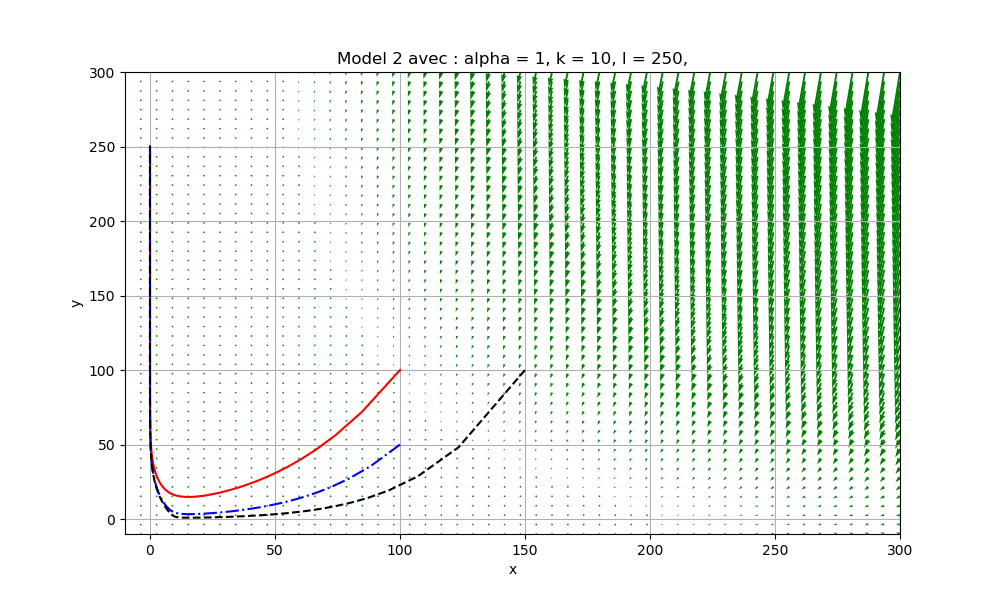
\includegraphics[width = 13cm]{y_predom2.png}\\
Comme pour le premier cas, on a choisi différentes conditions initiales. Pour que l'espèce y puisse prendre le dessus, il a fallu prendre une valeur de k nettement inférieure. $(x(t),y(t)) \longrightarrow (0,l) $. Il faut avoir un petit nombre d'individus de x (<25) pour que l'espèce y puisse progresser.

\subsubsection{Troisième cas}
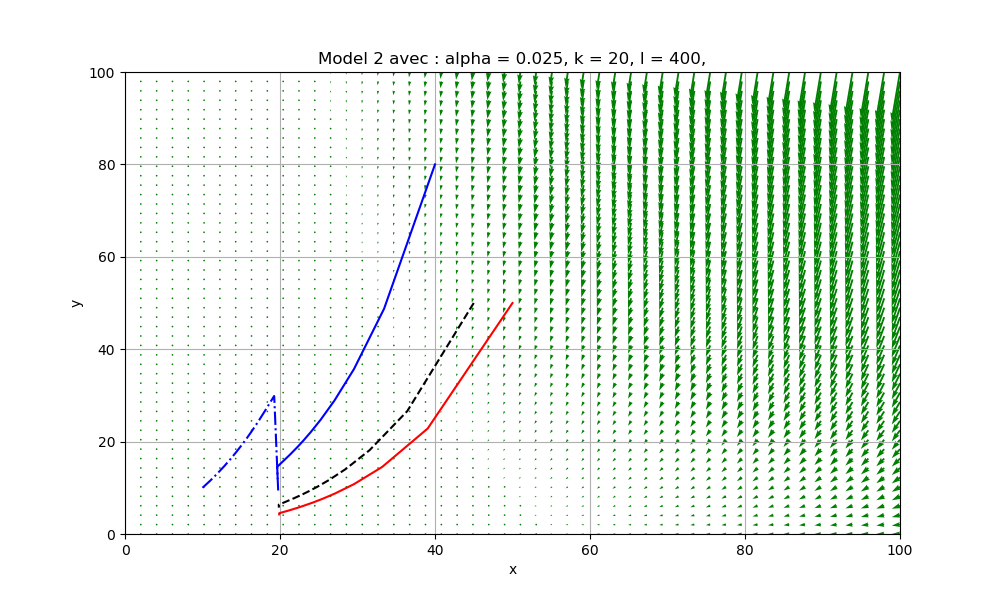
\includegraphics[width = 13cm]{point_stable3.png}\\
Dans ce cas, nous avons choisi les valeurs du paramètre a idéale pour que les courbes convergent vers le dernier point critique. On remarque qu'il y a coexistence entre les deux espèces. Cette situation est rendue possible lorsque l'espèce x a suffisamment de ressources pour se maintenir dans le milieu, mais pas assez pour prendre le dessus sur l'espèce y. $(x(t),y(t)) \longrightarrow (k-ay,l-x^2)$

\subsubsection{Quatrième cas}
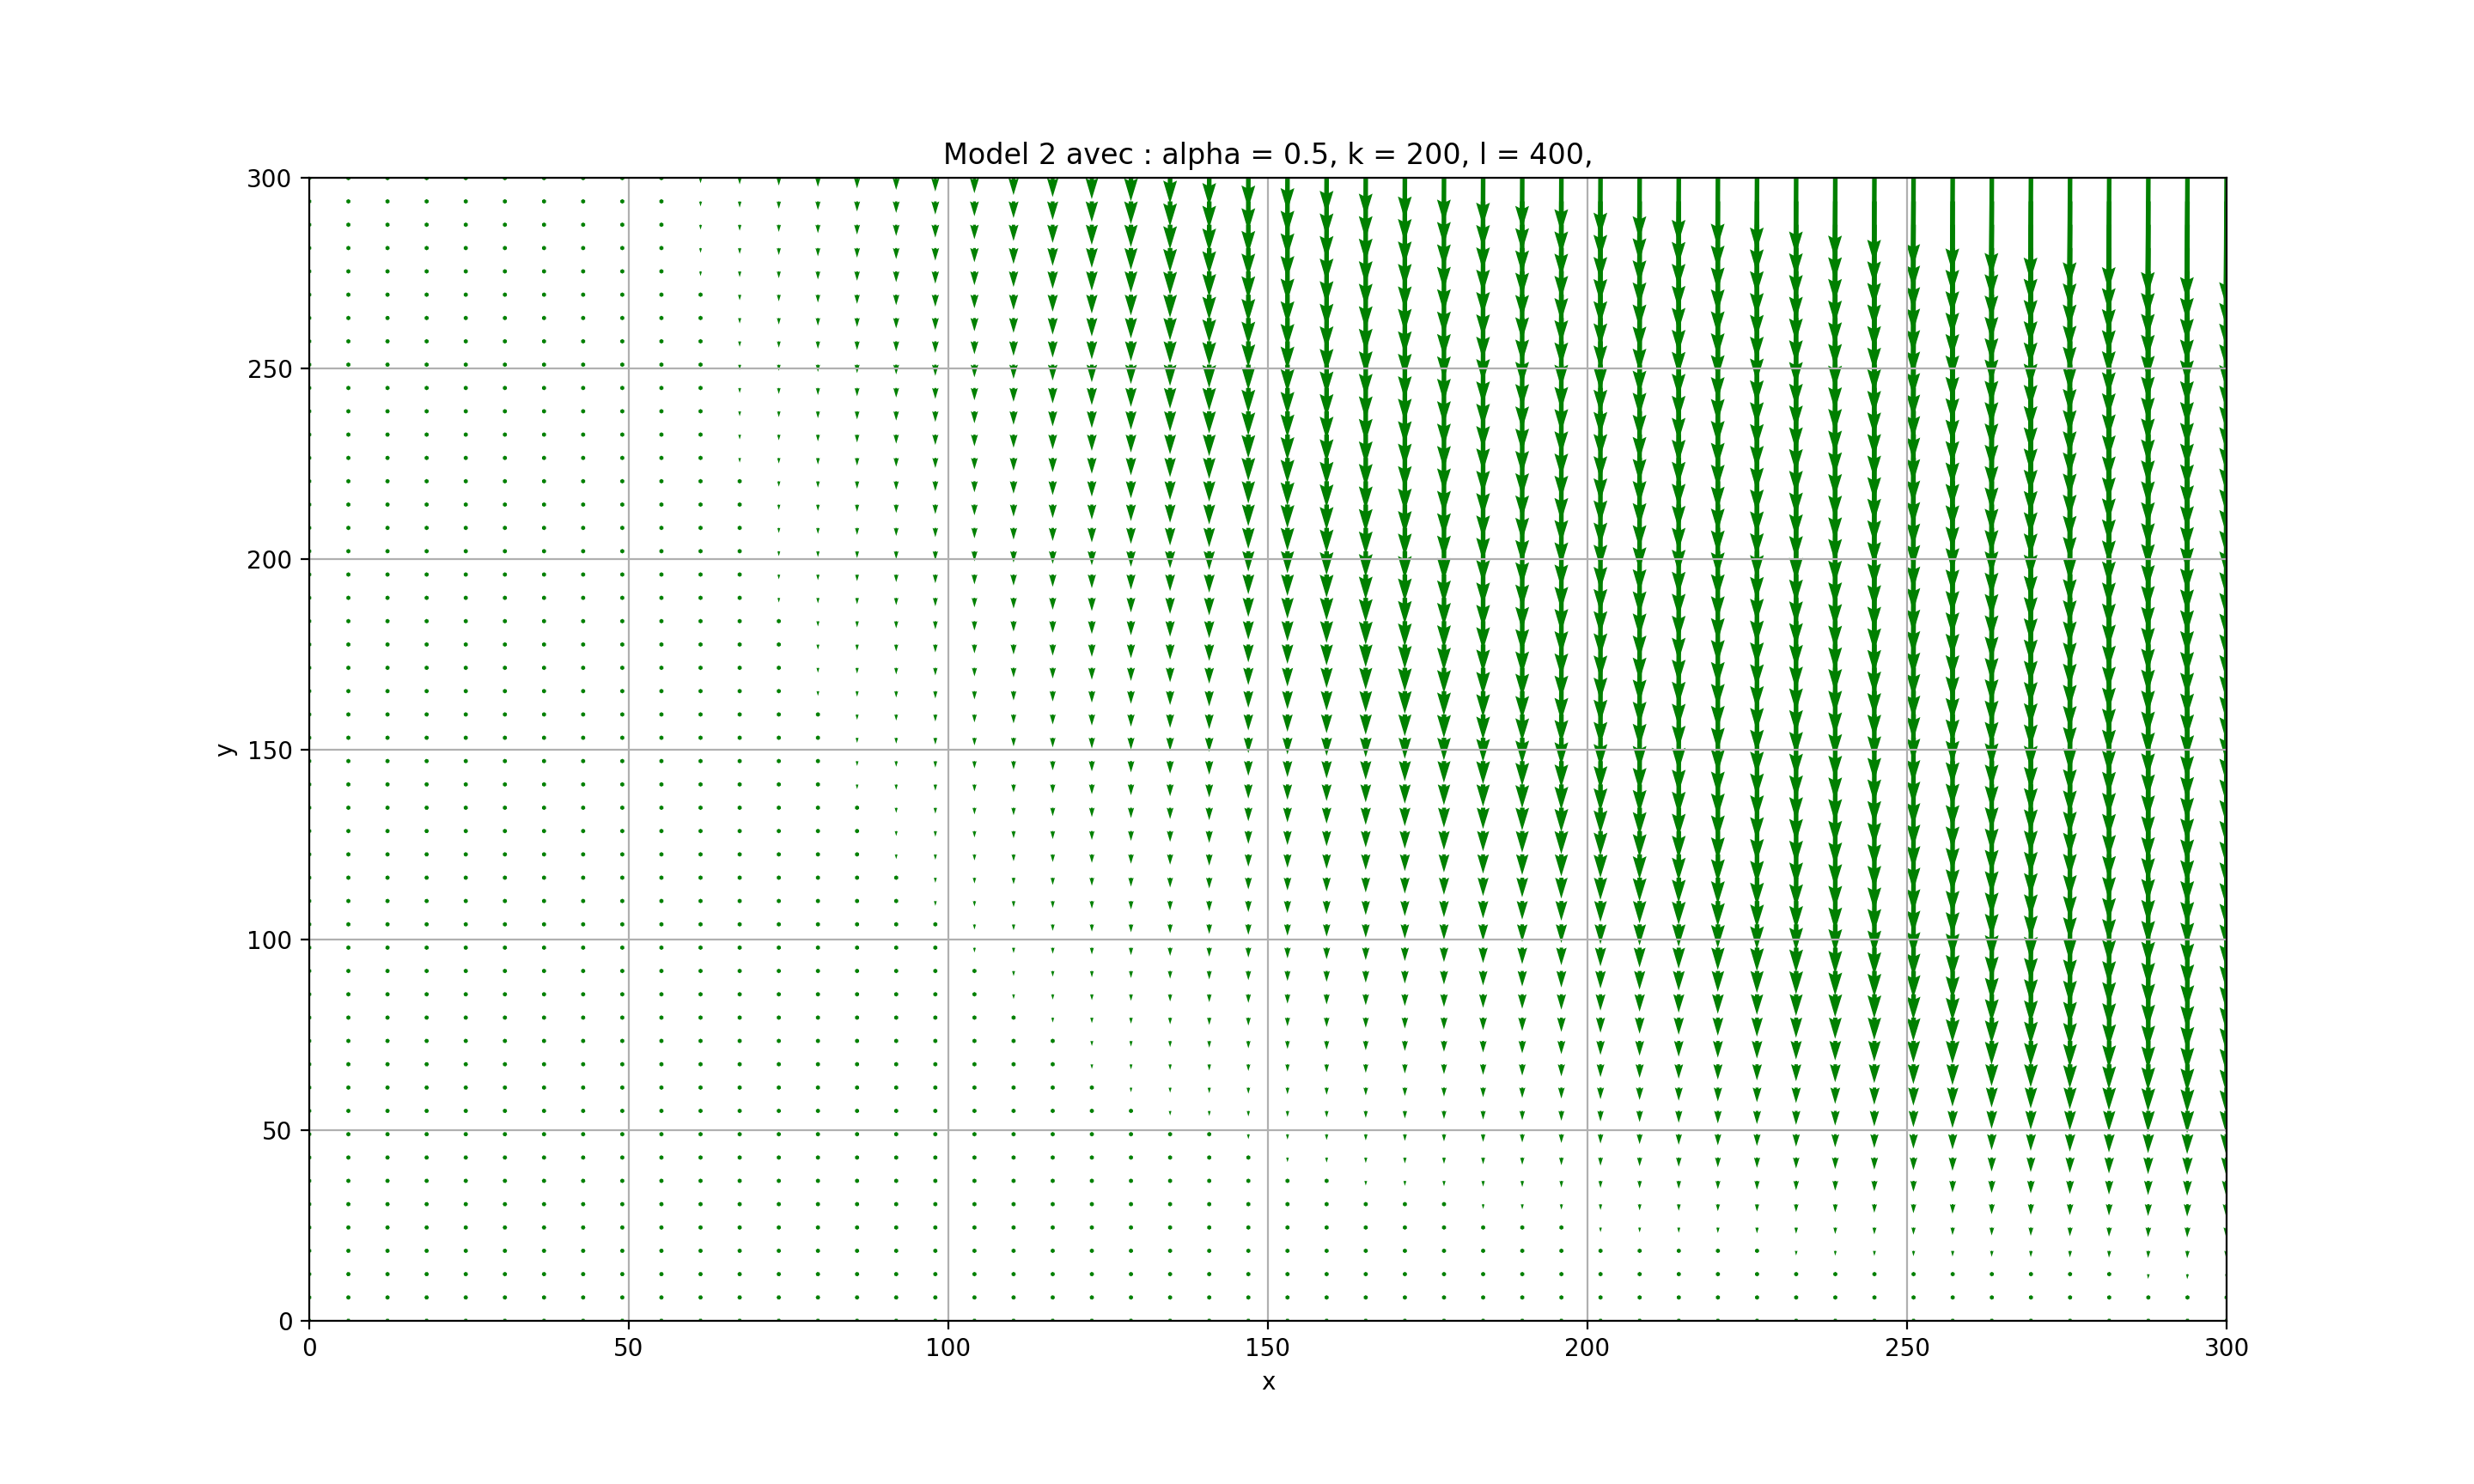
\includegraphics[width = 12.5cm]{figure_pf.png}\\
Pour ce cas là, nous avons choisi de mettre comme conditions initiales les points fixes trouvés lors de l'analyse de la stabilité du système: $(0,0)$, $(0,l)$ et $(k,0)$. Comme on peut le constater sur la figure ci-dessus, il n'y pas de courbes car comme nous l'avons bien démontré le système ne varie pas dans ce cas là.

\setcounter{secnumdepth}{1}
\subsection{Synthèse des résultats}
À partir des graphes obtenus et en les comparant aux résultats théoriques obtenus, nous voyons bien qu'ils sont concordants. En effet, avec des conditions initiales aléatoires et différentes, on a bien une convergence vers les points fixes. Aussi, en partant de ces points là, le système ne varie absolument pas (x'=0 et y'=0)\\

\section{Limites et amélioration du modèle}
\subsection{Remarques et interprétation}
Nous avons analysé la stabilité d'un système modélisant deux espèces en compétition. On remarque qu'il est très rare que ce genre de système se retrouve en équilibre. Il existe quelques point stables,\\respectant plusieurs conditions, pour les quels les deux espèces cohabitent. Pour des conditions initiales aléatoires, l'une des deux espèces prend le dessus, faisant disparaître l'autre. L'identification de l'espèce dominante dans le milieu dépend de ses ressources (k,l) mais surtout du paramètre a. Nous allons illustrer cette analyse et les différentes issues possible par des graphes. Concernant le modèle, on remarque que l'une des deux espèces est nettement avantagée: 

\begin{equation*}
\tag{S}
\left\{
\begin{array}{ll}
    \frac{dx}{dt} =  x(1 - \frac{x}{k} - \frac{a y}{k}) \\
    \frac{dy}{dt} = y(1- \frac{y}{l} - \frac{x^{2}}{l})
\end{array}
\right.
\end{equation*}\\

On remarque que la population x est avantagée car elle contribue grandement à la diminution de ressources dans le milieu l (par le terme $\frac{-x^2}{l}$. Cela influe directement sur le comportement du modèle, dans lequel la population de l'espèce x subsistera dans la plupart des cas. Rendant difficile la probabilité de trouver un point d'équilibre. \\\\

\begin{center}
    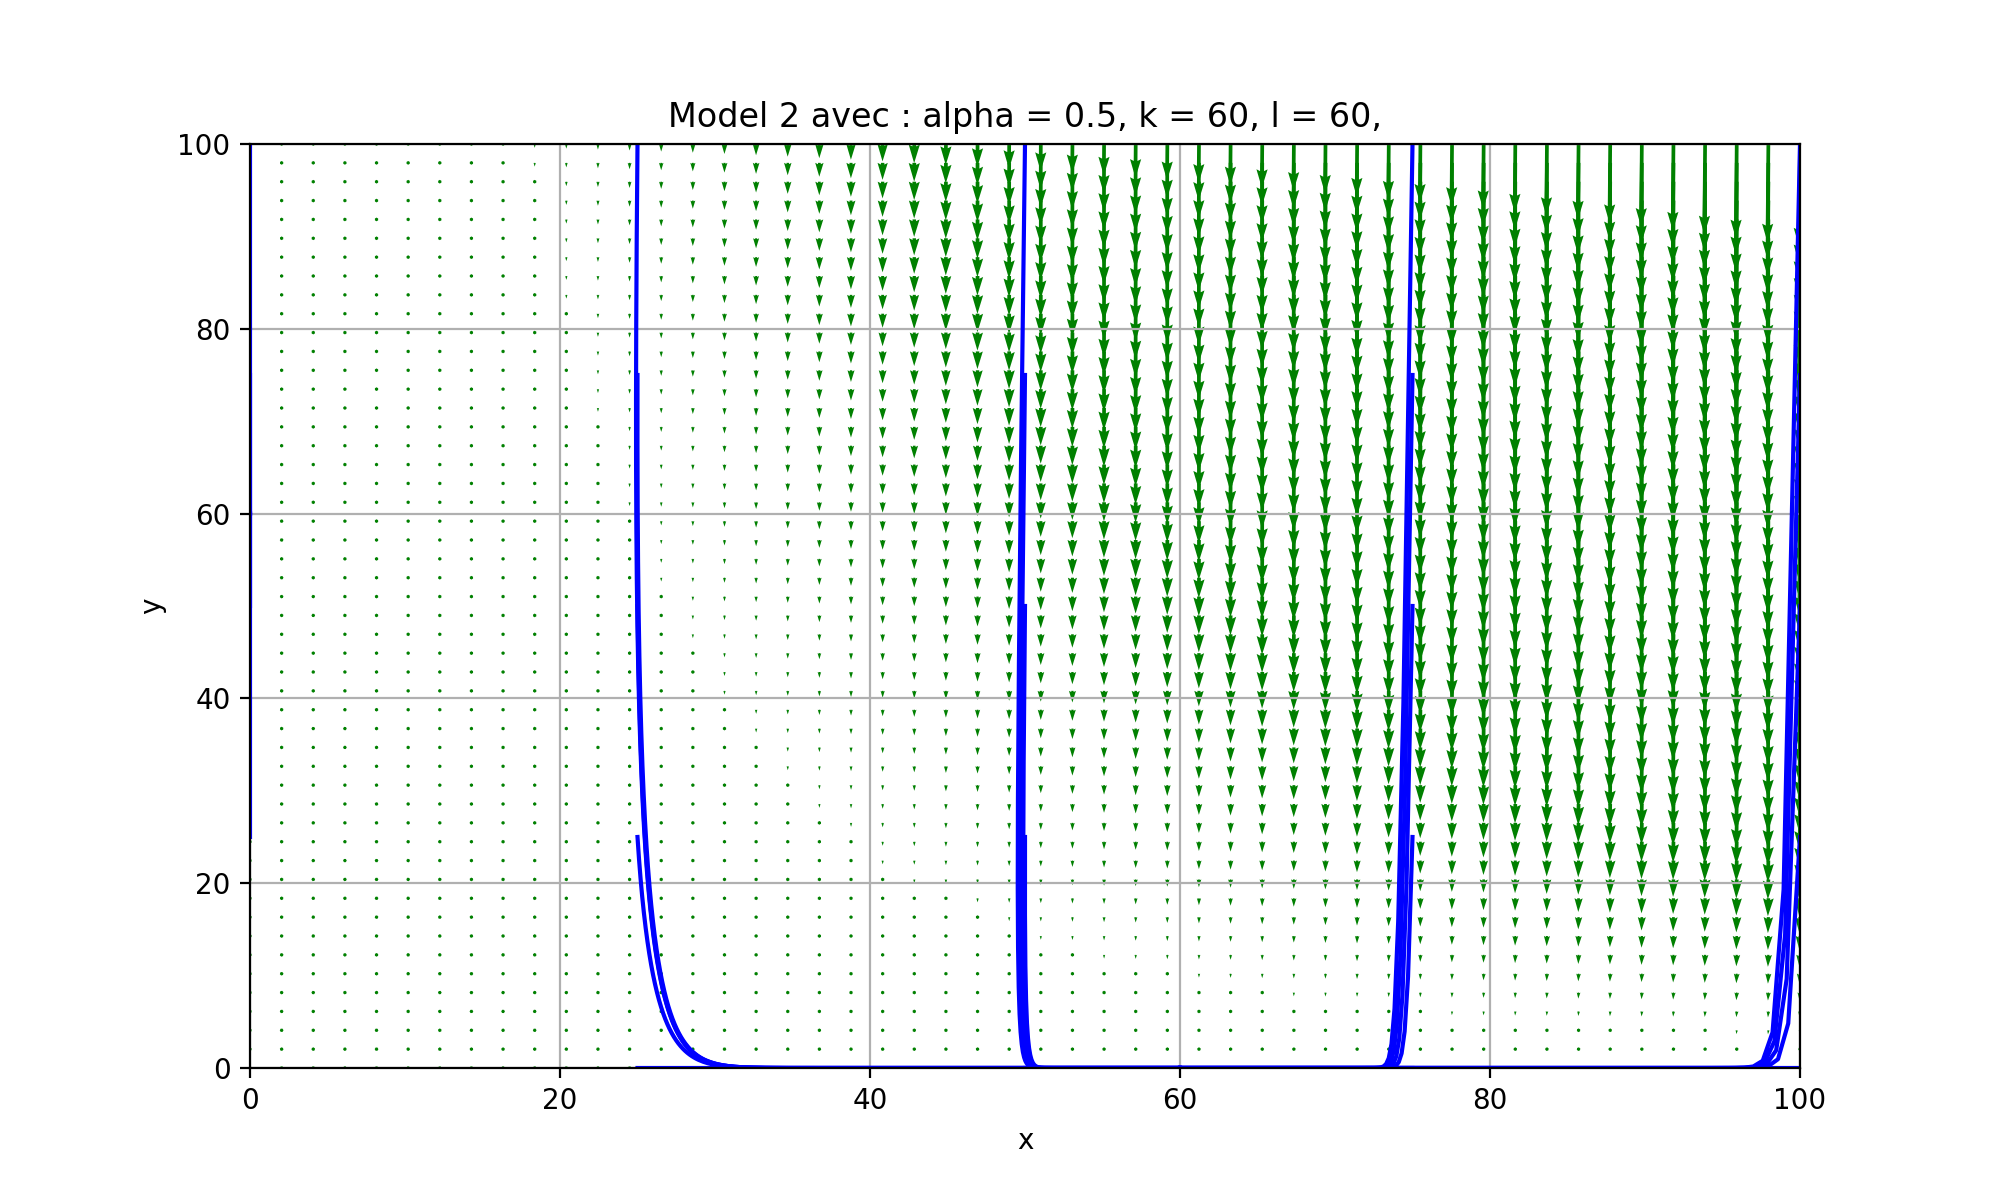
\includegraphics[width = 13cm]{Diagramme Phase Model_2.png}
\end{center}
Le diagramme de phase montre que la population de y tend à disparaître dans la grande majorité des cas. Ce modèle montre clairement un déséquilibre entre deux populations en compétition dans un milieu adapté à l'une d'entre elle. Ce modèle peut très bien représenter la sélection naturelle. Nous avons une disparition de l'espèce la moins adaptée au milieu, et une occupation massive du milieu par l'autre.

\subsection{Possible amélioration pour tendre vers la stabilité}
On propose un modèle "plus équilibré" en ajoutant un paramètre $b$ définissant la part d'individus de l'espèce x, se nourrissant de la quantité $l$.

\begin{equation*}
\left\{
\begin{array}{ll}
    \frac{dx}{dt} =  x(1 - \frac{x}{k} - \frac{a y}{k}) \\
    \frac{dy}{dt} = y(1- \frac{y}{l} - \frac{b x}{l})
\end{array}
\right.
\end{equation*}\\
\noindent
Avec ce modèle, on aurait plus de chance d'avoir une coexistence entre les deux espèces. Voici un aperçu du diagramme de phases du modèle proposé. On remarque qu'il y a convergence vers le point d'équilibre (40,40 )dans la plupart des cas\\
\begin{center}
    \includegraphics[width = 13cm]{Model_proposé.png}
\end{center}\\
Il 

\newpage
\setcounter{secnumdepth}{0}
\section{Conclusion}
Nous avons donc étudié le système donné en fonction de ses trois paramètres k, l et a. Nous avons pu analyser le comportement des deux espèces en compétition dans leur milieu de vie en identifiant l'impact de chaque paramètre ainsi que celui des conditions initiales choisies. En effet, la stabilité de la communauté étudiée dépend non seulement des paramètres du système mais aussi des conditions nécessaire à l'existence de celle-ci.
\begin{itemize}
    \item L'analyse mathématique nous a permis de déterminer les points fixes du système considéré ainsi que d'identifier sa stabilité.
    \item Notre code Python nous a permis de mettre en oeuvre notre interprétation en obtenant les graphes ainsi que les portraits de phases et donc d'évaluer nos résultats théoriques.
\end{itemize}
Grâce à notre application, nous avons étudié en détail l'évolution de chacune des deux espèces. Ce type de programme peut être très utile pour étudier le comportement de différentes populations en compétition, il pourrait comprendre l'évolution des espèces, notamment en étholoogie.

\vfill
\section{Liens et références}
\begin{itemize}[label=\textbullet]
    \vspace{0.3cm}
    \item Calcul Différentiel - MAIN | Cours de Myriam Comte - Chapitres 2 \& 3\\
    \item TP $n^o$ 3 de Python dirigé par Hacene Ouzia
\end{itemize}
\vfill \vfill

\newpage
\section{Annexes}
 - Diagramme UML de l'application Python utilisée :\\
\begin{center}
    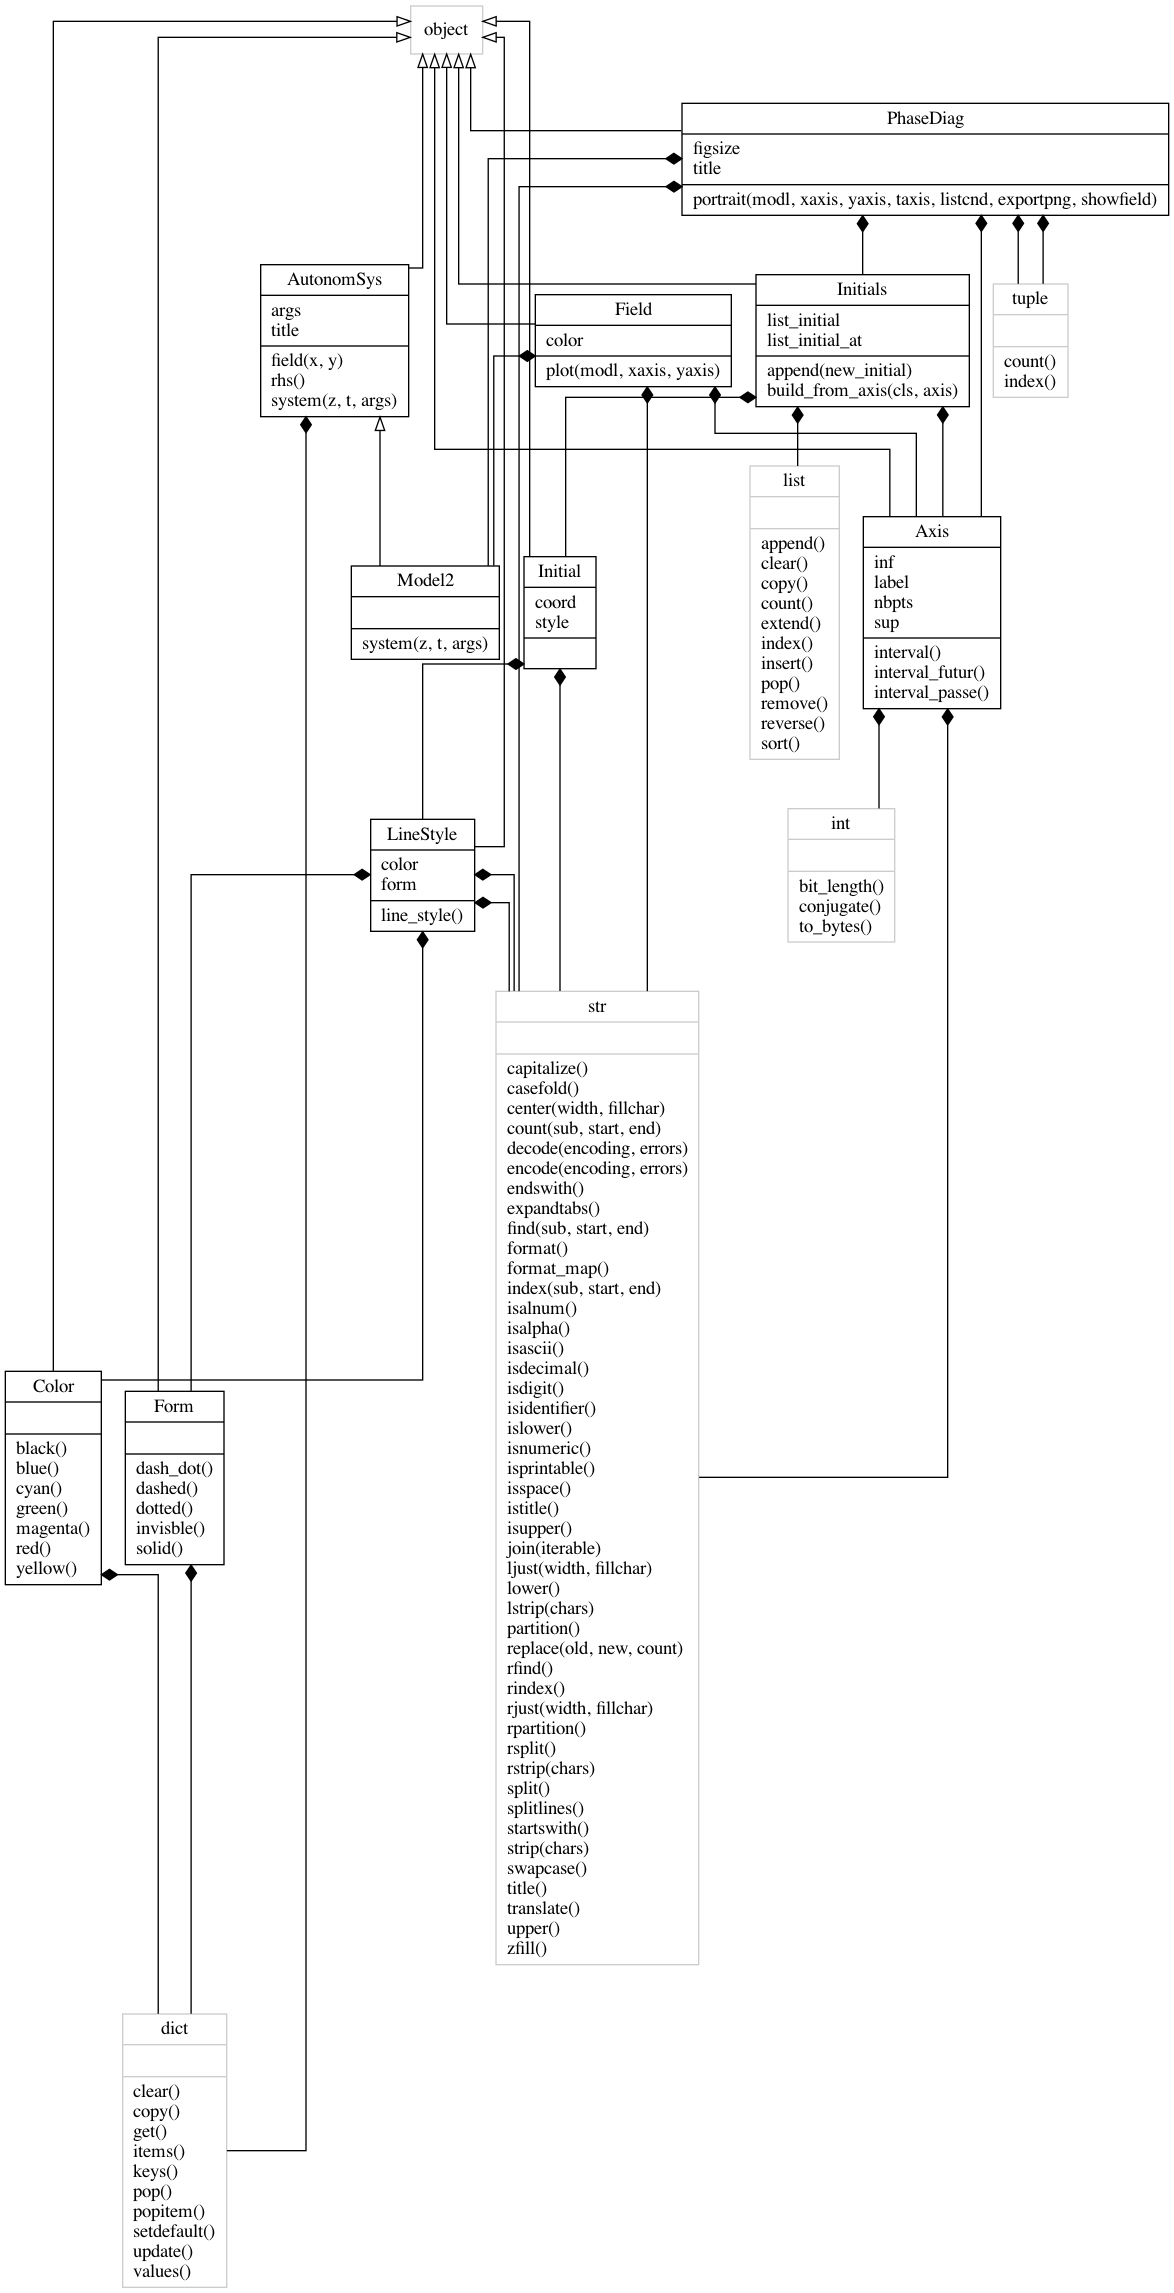
\includegraphics[height = 19cm]{UML_test.png}\\
    \footnote{Les classes de notre application sont en noir alors que celle du système sont en gris.} 
\end{center}

\end{document}
